\documentclass[tikz,border=5pt]{standalone}
\usepackage{amsmath,amssymb,hyperref}
\newcommand{\Spec}{\operatorname{Spec}}
\newcommand{\bT}{\mathbf{T}}
\begin{document}

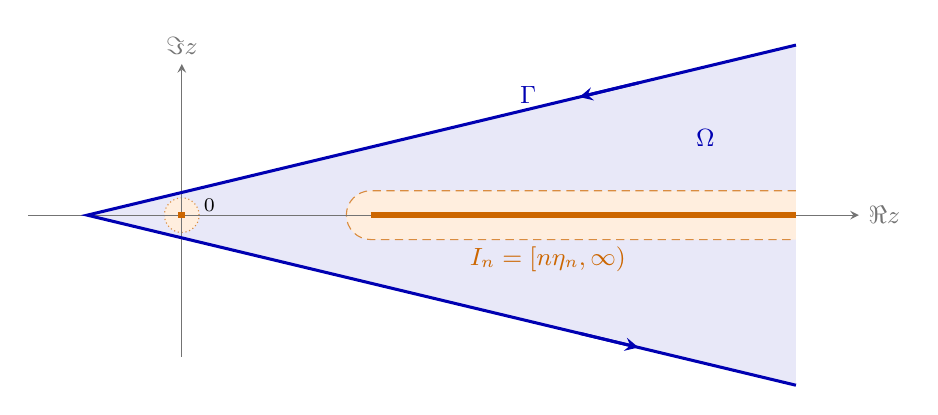
\begin{tikzpicture}[x=1cm,y=1cm,font=\small,>=stealth]
\colorlet{filterblue}{blue!70!black}
\colorlet{filterorange}{orange!80!black}
% The spectral ray starts at 2.4; its tubular neighborhood has radius 0.31.
\fill[filterblue!9] (-1.20,0)--(7.8,2.16)--(7.8,-2.16)--cycle;
\fill[orange!13] (7.8,.31)--(2.4,.31) arc[start angle=90,end angle=270,radius=.31]--(7.8,-.31)--cycle;
\draw[filterorange!75,densely dashed] (7.8,.31)--(2.4,.31) arc[start angle=90,end angle=270,radius=.31]--(7.8,-.31);
\filldraw[fill=orange!13,draw=filterorange!75,densely dotted] (0,0) circle[radius=.22];
\draw[->,black!55] (-1.95,0)--(8.6,0) node[right] {$\Re z$};
\draw[->,black!55] (0,-1.8)--(0,1.92) node[above] {$\Im z$};
\node[right,inner sep=1pt,font=\scriptsize] at (.24,.13) {$0$};
\draw[filterorange,line width=2.4pt] (2.4,0)--(7.8,0);
\fill[filterorange] (-1.2pt,-1.2pt) rectangle (1.2pt,1.2pt);
\node[below,text=filterorange,inner sep=2pt] at (4.65,-.32) {$I_n=[n\eta_n,\infty)$};
% Positive orientation keeps the sector to the left of each oriented ray.
\draw[filterblue,line width=1.1pt] (7.8,2.16)--(-1.20,0)--(7.8,-2.16);
\draw[filterblue,line width=1.1pt,->] (5.80,1.68)--(5.05,1.50);
\draw[filterblue,line width=1.1pt,->] (5.05,-1.50)--(5.80,-1.68);
\node[above,text=filterblue,inner sep=2pt] at (4.40,1.344) {$\Gamma$};
\node[text=filterblue] at (6.65,.98) {$\Omega$};
\end{tikzpicture}

\end{document}
